
\documentclass{../templates/llncs}
\usepackage{../templates/salt-light}
\usepackage{makeidx}
\usepackage{url}
\usepackage{graphicx}

\begin{document}

%\title{Vapour, a scripting approach to implement HTTP best practices}
%funny title???
%Cooking HTTP content negotiation with Vapour
%HTTP pressurizing with Vapour
%Vapour as a HTTP steam engine

\title{Cooking HTTP content negotiation with Vapour}

%TODO list:
% - decide the final title of the paper
% - find work related to cite it


\author{Diego Berrueta\inst{1}, Sergio Fern\'andez\inst{1} and Iv\'an Frade\inst{2}}

\institute{
Fundaci\'on CTIC\\
Gij\'on, Asturias, Spain\\
\email{\{diego.berrueta,sergio.fernandez\}@fundacionctic.org\\http://www.fundacionctic.org/}
\and
Universidad de Oviedo\\
Oviedo, Asturias, Spain\\
\email{ivan.frade@gmail.com\\http://www.uniovi.es/}
}

\maketitle

\begin{abstract}
The Semantic Web is built upon a distributed amount of knowledge published on 
the Web. But this vision can not be implemented without some basic norms and 
rules of publishing and making machine-understandable all this data. Special 
mention must be given the publication of RDF vocabularies for the importance that
they have in the Semantic Web architecture. In this paper we describe a light 
scripting web-based application that validates some of these rules. We think 
that practical experimentation permits illustrating and discussing some
problems of these mechanisms.
\end{abstract}

\section{Introduction}

The Semantic Web is a big container, a universal medium for data, information
and knowledge exchange. However the Semantic Web is not only about putting data on
the Web, it is something more. There are necessary some basic rules to follow
in order to get a useful knowledge from all this Linked Data. Tim Berners-Lee %review it
outlined four principles~\cite{TimBL2006} of how to publish linked data on the 
Web~\cite{PublishLinkedData2007}. Could be summarized as that you must use 
\texttt{URIs}~\cite{RFC3986} as names and provide useful information where you 
could be discovered more information. But cool URIs~\cite{Sauermann2007} are 
not enough, you also need to provide the best representation expected in each
request for each kind of agent, human or software.

On the Web, the documents are requested using HTTP~\cite{HTTP} as protocol. It 
provides a mechanism known as \textit{content negotiation}. Using this mechanism 
it is possible to offer Web content in better format or languages requested. 
Use transparent content negotiation in HTTP~\cite{Holtman1998} has many 
benefits~\cite{Seshan1998}, but must be implemented carefully if you do 
not want to make some mistakes, as we could see with more detail in 
Section~\ref{sec:contentnegotiation} of this paper. Section~\ref{sec:vapour} presents 
a scripting application for the Semantic Web that helps in the task of implement 
HTTP content negotiation correctly. Finally, in Section~\ref{sec:conclusions} 
we present some conclusions and future work.


\section{\label{sec:contentnegotiation}Content negotiation with Apache: Recipes}

%FIXME: something generic about content negotiation
%an image explaining content negotiation?
%something like http://www.w3.org/TR/cooluris/img20071212/303.png

Apache HTTP Server, probably the most used Web server now, mainly provides three ways 
to implement content negotiation\footnote{\url{http://httpd.apache.org/docs/2.0/content-negotiation.html}}, 
each one with a different approach:

\begin{description}

  \item \textbf{Type Map:} Explicit handlers are described in a file (.var) for 
        each resource. The necessary configuration is quite complicated and 
        tedious, so probably that is the reason because it is hardly used.

  \item \textbf{MultiViews:} Based in the MIME-type of the files, MultiViews 
        delegates in Apache the task of choosing the best file in the current 
        directory to serve when the resource requested does not exist. It adds 
        an additional header (\texttt{Content-Location}) indicating the direct 
        location of the file served. Could also be extended using 
        \texttt{mod\_mime}\footnote{\url{http://httpd.apache.org/docs/2.0/mod/mod_mime.html}}
        to associate concrete handlers to other file extensions. But this solution
        has a quite important problem: it only works in the same directory.

  \item \textbf{Rewrite request:} Probably because the both methods previously 
        presented do not work as expected, the most currently used is another 
        that is not designed specifically for content negotiation tasks. This
        mechanism uses the module 
        \texttt{mod\_rewrite}\footnote{\url{http://httpd.apache.org/docs/2.0/mod/mod_rewrite.html}}
        to rewrite the request according some mandatory ad-hoc rules and redirect,
        using HTTP 30X status codes, to the appropriate URI. Obviously it loses 
        some time with the extra HTTP round-trip, but it is negligible.

 \end{description}

The W3C has published \textit{Best Practice Recipes for Publishing RDF Vocabularies}~\cite{Recipes},
a document with several recipes that show how to publish RDF/OWL Vocabularies using
mainly the last mechanism described. It provides step-by-step instructions for publishing 
vocabularies on the Web, giving example configurations designed to cover the most 
common cases. It's a really useful document to help to publish the vocabularies.

But it is not perfect, and still there is an important issue to 
solve\footnote{\url{http://www.w3.org/2006/07/SWD/track/issues/58}}: 
``the recipe for responding to an accept header only responds to a header which
EXACTLY matches''. Consider cases like \texttt{application/rdf+xml;q=0.01} or 
\texttt{text/*} or combinations of such patterns. This is a very serius problem
with not an easy solution. Probably might be solved by moving from \texttt{mod\_rewrite}
to \texttt{mod\_negotiation}\footnote{\url{http://httpd.apache.org/docs/2.0/mod/mod_negotiation.html}},
or with a combination of both techniques.

%FIXME: solution ISSUE #58 !!!
%http://lists.w3.org/Archives/Public/public-swd-wg/2007Jul/0177.html

\section{\label{sec:vapour}Vapour, a scripting approach to debugging content negotiation} 
%FIXME: find a better title for this section

As we can see, the Recipes are not perfect. Futher testing the results of content 
negotiation can become fairly complex for some of them. Obviously, you could do 
it manually with help of some tools, such as 
cURL\footnote{Richard Cyganiak's explanation of how to use cURL to debug content negotiation, 
blog post available at: \url{http://dowhatimean.net/2007/02/debugging-semantic-web-sites-with-curl}}
or socat\footnote{\url{http://www.dest-unreach.org/socat/}}
But it is not a very handy way, specially when you need to do intensive tests over your 
configuration.

\begin{figure}
 \centering
 \includegraphics[width=12cm]{images/report-summary.png}
 \caption{\label{fig:report-summary}Example of a report summary made by Vapour.}
\end{figure}

In order to facilitate the testing of the results of content negotiation on a single 
URI, we developed a web-based application called Vapour\footnote{\url{http://vapour.sourceforge.net/}}
that facilitates the task. This service will request the provided vocabulary 
URI fromthe server multiple times (namespace, a class and a property), run a 
test suite specifically designed to test the responses of the server against 
the Recipe specifications. According to these tests, the system suggests you the 
best recipe/s for your server configuration. It is built upon an RDF store %(in memory)
that stores all assertions. It uses a combination of EARL~\cite{EARL}, HTTP
Vocabulary~\cite{Koch2007} and an RDF representation of the Recipes. Thus Vapour 
is able to provide reports both in HTML and in RDF~\cite{RDF}. For (X)HTML view 
the service displays a clean and concise pass/fail report on each set of tests 
as  well as a detailed explanation of its  findings (Figure~\ref{fig:report-summary}), 
including a graphical representation of the HTTP dialog used in each test.
For RDF view %,obviously using content negotiation (FIXMEEEEEEEEEEEEEEEEEE)
the system provide a RDF/XML serialization of the same report.

An online demo\footnote{\url{http://idi.fundacionctic.org/vapour}} of the project
is available to test it.

The application has been developed in the Python scripting language, using common
Python libraries such as urllib, httplib, web.py and RDFLib. Scripting languages as
Python allow an agile development of applications in record time with little resources. 
Its source code is also available in the project in SourceForge\footnote{\url{http://sourceforge.net/projects/vapour/}} 
as open source, licensed under the terms of the W3C Software License.

\begin{figure}
 \centering
 \includegraphics[width=12cm]{images/arch.png}
 \caption{\label{fig:arch}High level architecture of Vapour.}
\end{figure}

As can be viewed in the Figure~\ref{fig:arch}, Vapour has a simple and functional
design that fulfils the concrete objectives of the project. It is composed of three
main components:

\begin{description}

  \item \textbf{cup} is the web front-end. It is built using web.py as framework
        and Cheetah as template engine. It provides a web interface that allows 
        the user to interact with the other components of the platform in a 
        simple way. Obviously, the system has been designed to allow more types 
        of interfaces and, for example, we also provide a command line interface.

  \item \textbf{teapot} is the core of the application. It implements each
        recipe of the W3C working draft, requesting necessaries HTTP dialogs 
        (with and without content negotiation) to evaluate each test with the 
        mime-types expected. It requests the URI of the vocabulary, and also the 
        URI of a class and on the URI of a property. All resulting assertions are 
        stored in the RDF store to be serialized later in the interface.

  \item \textbf{strainer} is the module in charge of generating the reports for
        each test performed. Basically it makes some SPARQL~\cite{SPARQL} queries
        on the model to obtain the trace of each test, and it generates the
        report in the format requested. For HTML reports we again use Cheetah 
        templates.

\end{description}

The service can be deployed as a normal CGI behind Apache or using a Python web 
framework. We reviewed the security of the application avoiding some common problems
in this kind of applications, such as limiting requests per client and refusing
request over resources located in private IP address ranges.

\section{\label{sec:conclusions}Conclusions}

Content negotiation is a dangerous technique. At the first appeareance is something very 
simple, but as we have seen it is too easy to make certain mistakes. This is 
further complicated when we have formats embedded within other formats,
such as RDFa~\cite{Birbeck2006}. Scripting languages, and applications such as 
Vapour, are very useful in solving some kind on tasks and provide quality 
assurance in the best possible way.

As we have seen, it is still necessary to solve as soon as possible some 
important issues in the actual document of the Recipes. While we do not 
find the most correct way to do it, maybe a \textit{push} action from Web 
community will be necessary to develop a new module that allows to serve 
Linked Data in the correct way with content negotiation.

The application presented in this paper is still a prototype, but a prototype 
that helps to debug how we use content negotiation in our servers. One of the 
goals was to provide an RDF serialization of the reports. Using this machine-readable 
format, it should be easy to deploy another service upon it that uses this data for 
another task: for example, a service to check the compliance of a specific collection 
of vocabularies published on the Web.


% ---- Bibliography ----
\bibliographystyle{abbrv}
\bibliography{../references}

\end{document}
